%------------------第三章---------------------------
    \newpage
	\section{超声波接近传感器硬件电路设计}
	
    \subsection{超声波接近传感器控制电路}
    本设计中所使用的CPLD芯片型号为EPM240T100C5N,涉及到的控制电路较简单,在最小系统板的基础上,增加了检测计数电路和TUSS4470外围电路。如图\ref{传感器整体原理图}为传感器整体的原理图,其中主要包括了电源模块、JTAG下载模块、检测计数模块、时钟模块以及复位模块。电源
    \begin{figure}[ht]
        \centering
        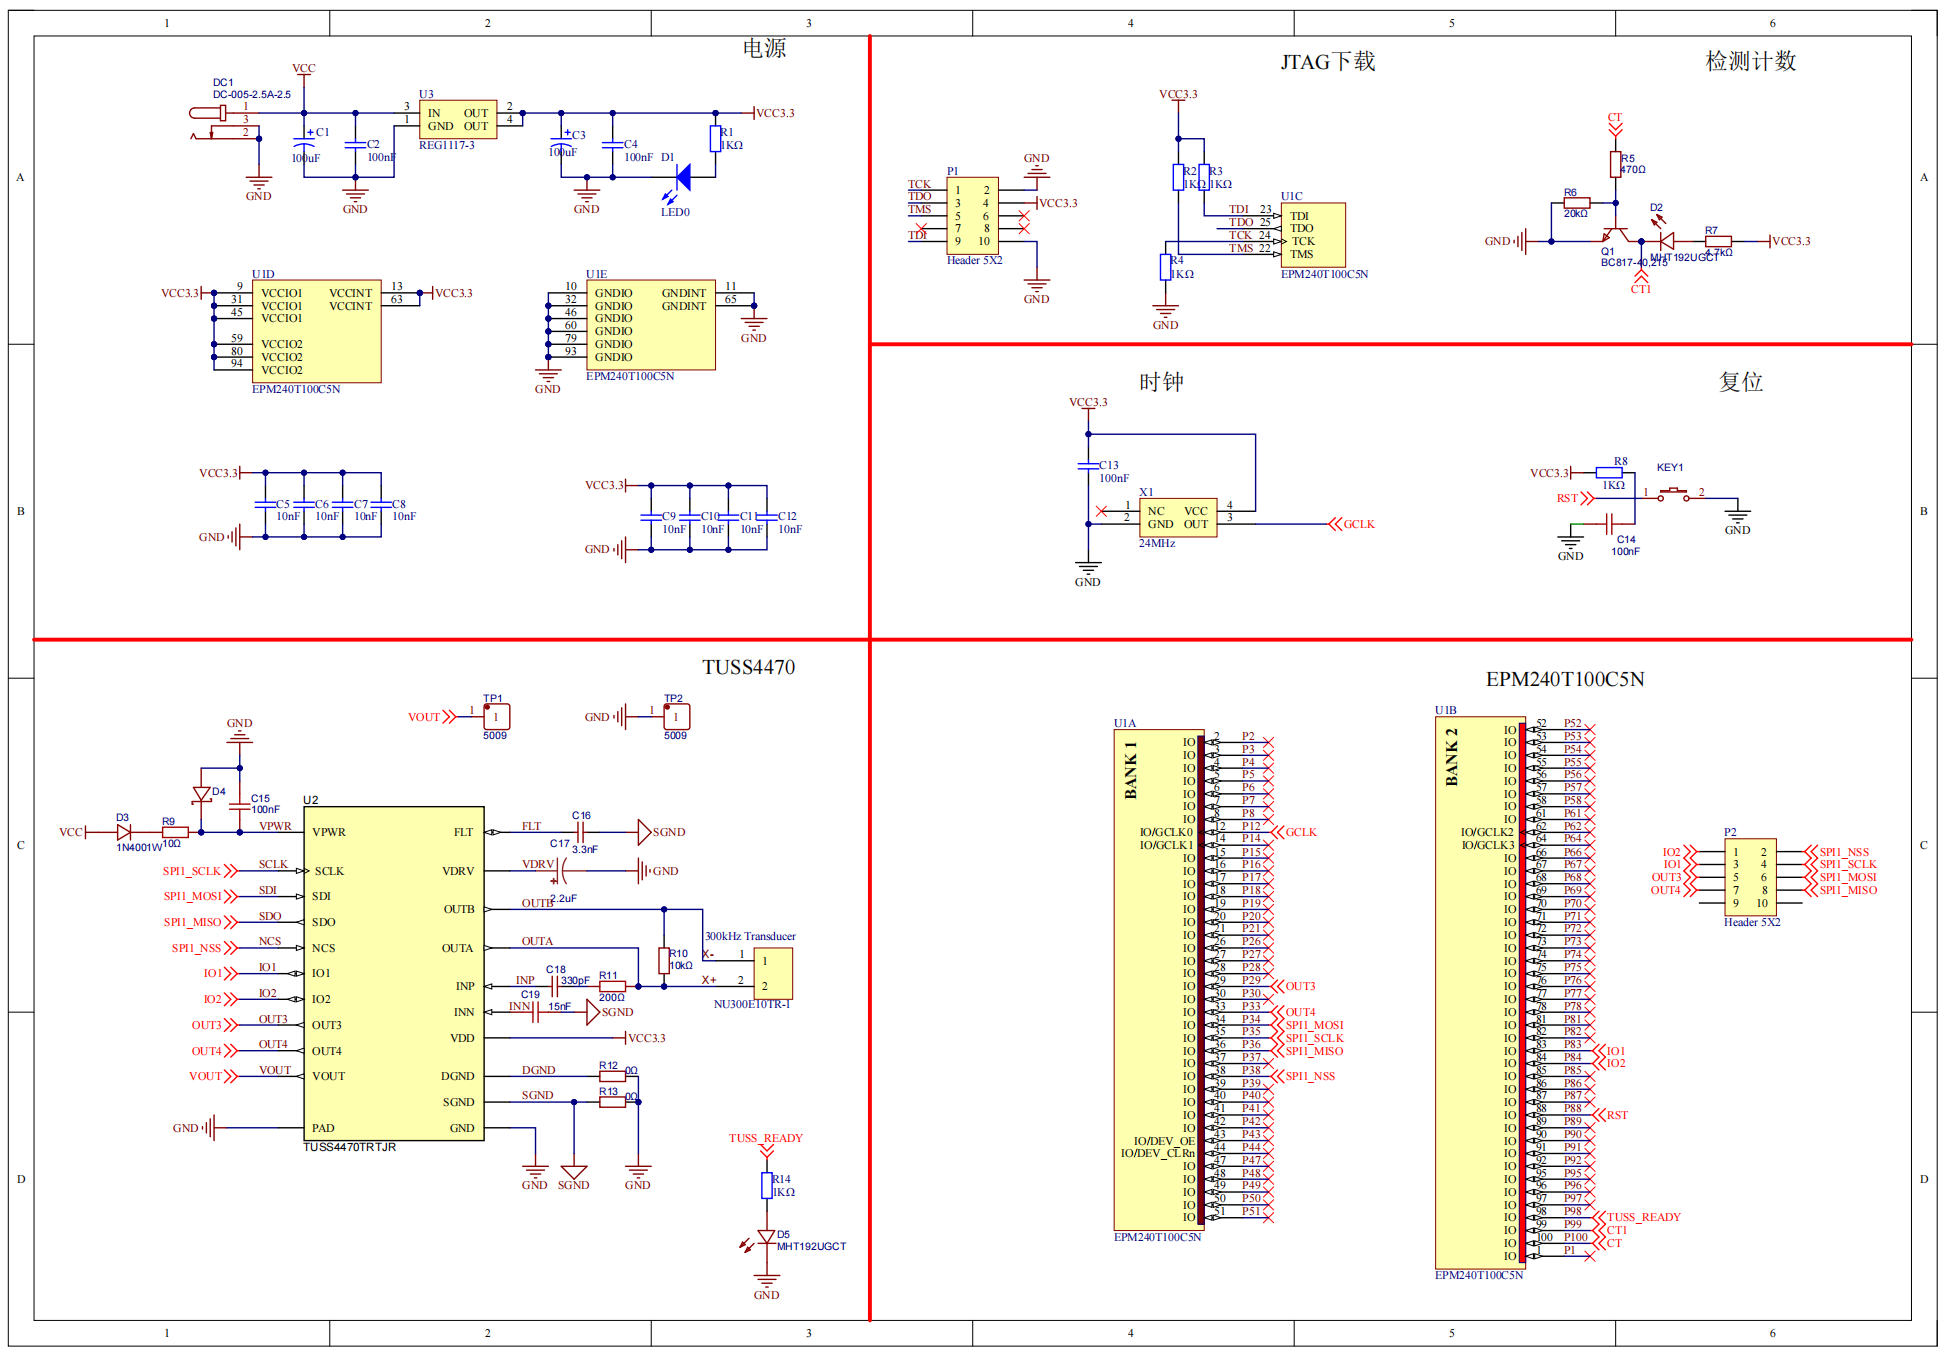
\includegraphics[width=12cm]{figure/Overall circuit.png}
        \caption{传感器整体原理图}
        \label{传感器整体原理图}
    \end{figure}
    \subsubsection{电源模块}
      根据查找芯片手册,可得知EPM240T100C5N的控制电压为:
    TUSS4470芯片的控制电压为3.3V
    超声探头的驱动电压为:5V-30V
    可得出电源的设计方案。电源由DC接口、降压芯片、滤波电容组成,可得到12V以及3.3V的电压为各模块供电。电源模块中还包括了一个红色LED指示灯,当模块正常工作时,LED灯就会被点亮。
    
    \subsubsection{JTAG下载模块}
    JTAG\upcite{JTAG}(Joint Test Action Group) 下载模块是一种用于编程和调试数字电路和嵌入式系统的通信接口。它通常由三个主要部分组成:JTAG控制器、JTAG下载模块和目标设备。JTAG下载模块的主要作用是将编译后的程序通过JTAG接口下载到目标设备中。其工作原理如下:
    
1、JTAG控制器通过JTAG接口向目标设备发送命令和数据,控制目标设备进入下载模式。

2、JTAG下载模块将编译后的程序通过下载接口发送到目标设备中,可以通过串行或并行方式进行数据传输。

3、目标设备接收到数据后,将其存储到相应的存储器中,如闪存、RAM等。

4、JTAG下载模块会根据设定的校验方式对下载数据进行校验,以确保数据的正确性。

5、下载完成后,JTAG控制器将目标设备从下载模式中退出,使其重新进入正常运行状态。

在本设计中JTAG主要用于下载烧录调试MCU代码。

    图\ref{JTAG下载模块电路图}左侧为JTAG接头,用于连接下载器,右侧为MCU芯片的连接图其中TCK引脚为测试时钟,
    TDI引脚为测试数据输入,
TDO引脚为测试数据输出,
TMS为测试模式选择,
因为只有一条数据线,通信协议有必要像其他串行设备接口,如SPI一样为串列传输。时钟由TCK引脚输入。配置是通过TMS引脚采用状态机的形式一次操作一位来实现的。每一位数据在每个TCK时钟脉冲下分别由TDI和TDO引脚传入或传出。可以通过加载不同的命令模式来读取芯片的标识,对输入引脚采样,驱动(或悬空)输出引脚,操控芯片功能,或者旁路(将TDI与TDO连通以在逻辑上短接多个芯片的链路)。
    \begin{figure}[ht]
        \centering
        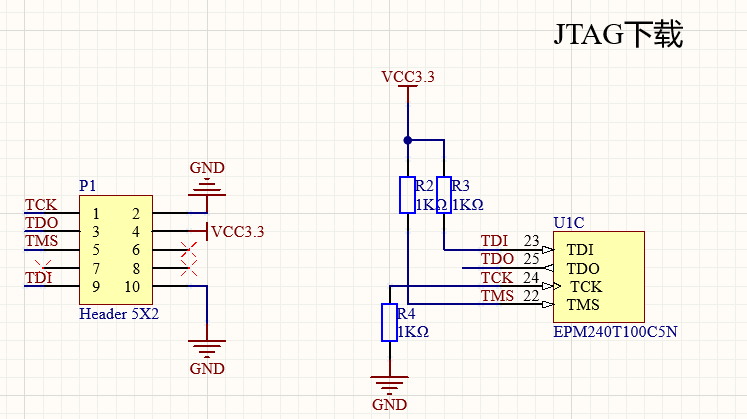
\includegraphics[width=7cm]{figure/JTAG download circuit.png}
        \caption{JTAG下载模块电路图}
        \label{JTAG下载模块电路图}
    \end{figure}
    
    \subsubsection{检测计数模块}
    检测计数模块的功能在于,亮灯提示钢化玻璃到位,并对经过的玻璃进行计数。如图\ref{检测计数模块电路图},CT引脚为MCU输出信号,当程序确定检测到物体后,CT引脚电压拉高,LED灯亮,当物体离开检测范围后,LED等灯灭。CT1引脚则是作为MCU的输入信号,当检测到一次物体后,CT1发出一次脉冲信号,计数加一,以此来实现计数功能。
    \begin{figure}[ht]
        \centering
        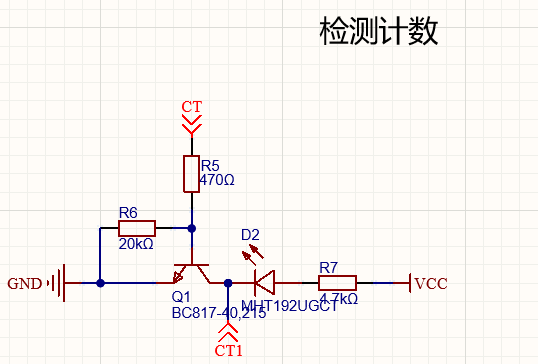
\includegraphics[width=7cm]{figure/detection count circuit.png}
        \caption{检测计数模块电路图}
        \label{检测计数模块电路图}
    \end{figure}
    
    \subsubsection{时钟模块}
    时钟模块用于生成稳定的时钟信号,是数字系统中非常重要的组成部分。时钟信号可以用于同步数字系统中各个模块的操作,确保数据在正确的时间传输和处理,从而提高系统的可靠性和性能。
    CPLD芯片的正常运行也需要时钟驱动,本设计选取27MHz的有源晶振作为外部时钟,从芯片的全局时钟引脚输入。
    
    \subsubsection{复位模块}
   CPLD芯片的复位电路一般采用外部复位电路,用于在系统启动时将芯片复位到初始状态,确保芯片能够正确运行,因此增加复位模块。通过查找芯片手册\upcite{CPLD芯片手册}得知,当拉低RST引脚的电压时,CPLD芯片将会产生复位信号,使芯片复位。
   
    
    \newpage
    \subsection{TUSS4470芯片外围电路}
    
    
    \begin{figure}[ht]
		\centering
		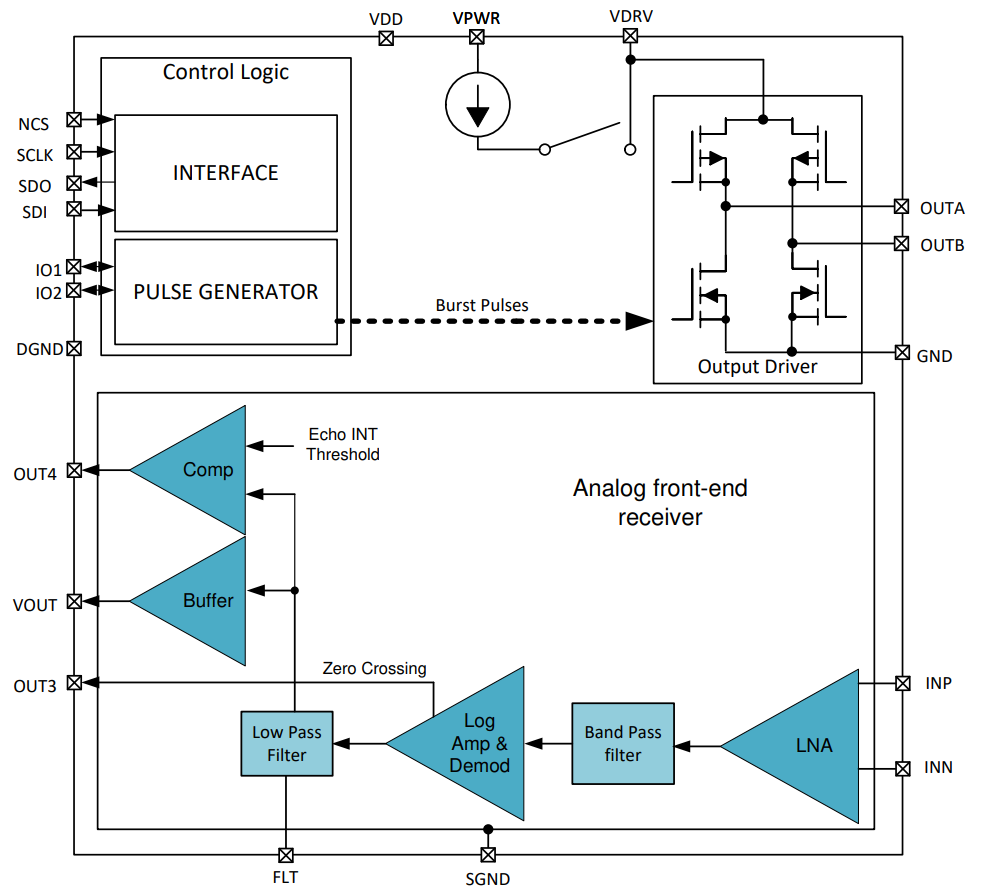
\includegraphics[width=12cm]{figure/Function Block Diagram.png}
		\caption{TUSS4470芯片功能框图}
		\label{TUSS4470芯片功能框图}%文中引用该图片代号
\end{figure}
 图\ref{TUSS4470芯片功能框图}为TUSS4470驱动芯片的整体功能框图\upcite{TUSS4470芯片手册},以此作为外围电路设计的参考资料。如图所示,芯片按照功能可分为逻辑控制、输出驱动、回波接收三个部分。其中逻辑控制部分又分为SPI通信和脉冲发生模块,SPI通信模块用于接收MCU芯片发送的芯片配置数据,脉冲发生模块的两个引脚IO1、IO2连接MCU芯片作为脉冲发生控制引脚,根据芯片不同的IO模式,两个引脚配合产生指定脉宽、脉冲数的脉冲信号;输出驱动模块的OUTA、OUTB引脚直接连接超声换能器,VDRV引脚连接外部电容,VPWR可对电容充电,在VDRV到达设定电压值后,VPWR停止对VDRV供电,这使得超声换能器的驱动电压可以保持在设定值,以此保证发出脉冲的声压水平可以稳定在一定水平,从而保证发射出稳定的脉冲波(其中VDRV的设定电压可通过SPI对芯片进行配置);回波接收模块的作用在于:对回波信号进行处理,输出可供MCU进行检测判断的信号其中INP、INN引脚连接超声波换能器的正负端,FLT连接外部电容作为低通滤波器对回波信号进行滤波处理。OUT3引脚内部连接至模块中的对数解调模块,当回波信号在模块内进完成放大进行解调时,将某阶段信号作为零点,输出过零信号,以验证接收信号的频率, 提高对其他信号的抗干扰性。OUT4作为检测到位的指示信号,当VOUT输出电压超过芯片配置数据中设定的阈值时,OUT4拉高。(VOUT引脚的电压值由公式\ref{VOUT公式}决定)。
  
    \begin{equation}
        V_{OUT}=G_{VOUT} \cdot SL_{LOG}\cdot20log_{10}(\frac{G_{LNA} \cdot G_{BPF} \cdot V_{IN}}{INT_{LOG} \cdot K_X})
        \label{VOUT公式}
    \end{equation}

        其中$G_{VOUT}$为对数放大器的斜率增益调整(Slope or gain adjustment),$SL_{LOG}$为对数运算放大器的斜率调整(slope of logarithmic amplifier),$G_{LNA}$为回波增益,$G_{BPF}$为0.9V/V,$V_{IN}$为INN引脚的输入,$INT_{LOG}$为对数放大器截距( logarithmic amplifier intercept),$K_X$为对数截距平差(log intercept adjustment)。\par
    回波接收模块的详细工作框图如图\ref{回波接收模块}所示。
    \begin{figure}[ht]
        \centering
        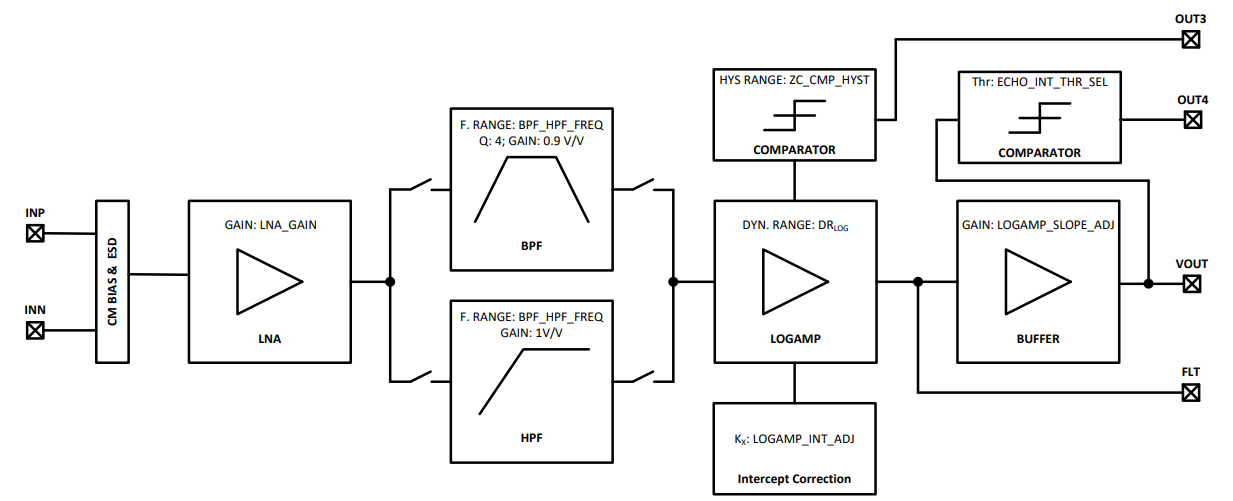
\includegraphics[width=10cm]{figure/Analog Front-End Block Diagram.png}
        \caption{回波接收模块}
        \label{回波接收模块}
    \end{figure}\par

    参考芯片手册相关内容,进行了TUSS4470芯片外围电路的设计,如图\ref{TUSS4470芯片外围电路}所示。
    \begin{figure}[ht]
        \centering
        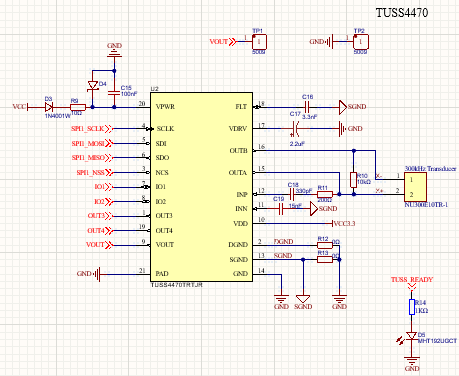
\includegraphics[width=10cm]{figure/TUSS4470 peripheral circuit.png}
        \caption{TUSS4470芯片外围电路}
        \label{TUSS4470芯片外围电路}
    \end{figure}
    \subsubsection{VOUT外接测试点}
    为方便后期调试,本设计将VOUT和GND作为外接测试点引出,可用电压表连接至两测试点测量VOUT电压。在设置完成传感器各参数后,根据实验测得在指定距离时VOUT引脚的的输出电压,并将其作为OUT4引脚比较的阈值,对芯片进行相关配置。

    \subsubsection{VPWR引脚电路}
    VPWR引脚输入电压范围为5V到36V,TUSS4470设备可能受到电池瞬变和反向电流的影响,因此采用外部组件保护芯片十分必要。图\ref{VPWR引脚}中除了靠近引脚的电容C15,二极管D3、D4和电阻R9就起到了保护芯片的作用。
     \begin{figure}[ht]
    	\centering
    	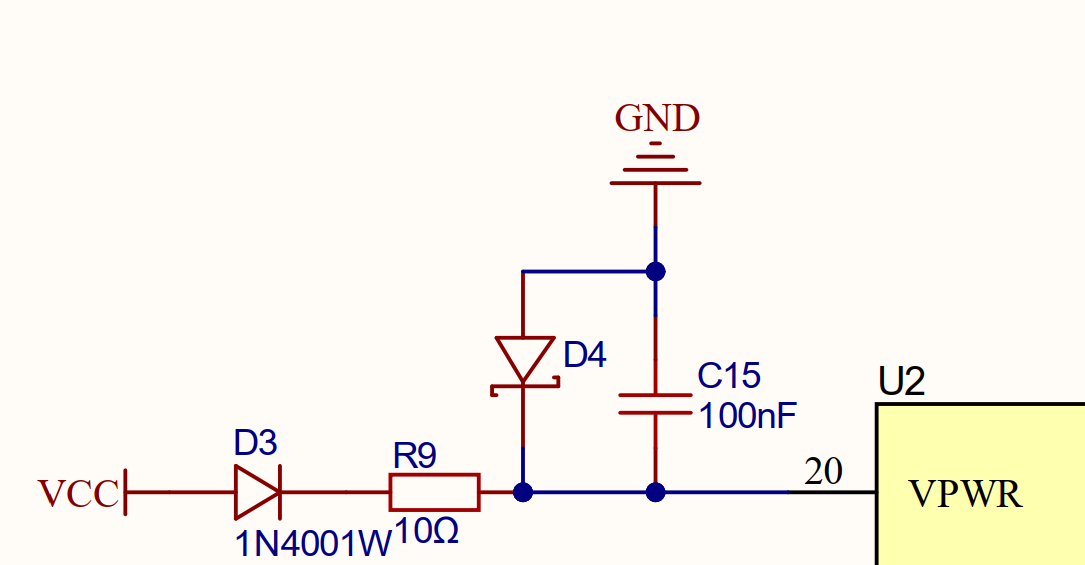
\includegraphics[width=10cm]{figure/VPWR PIN.png}
    	\caption{VPWR引脚电路}
    	\label{VPWR引脚}
    \end{figure}
    
    \subsubsection{FLT外接滤波电容}
    FLT引脚外接滤波电容,对应图\ref{TUSS4470芯片功能框图}回波检测模块中的低通滤波器。该滤波电容的作用在于,去除对数放大器输出中的高频信号,使解调包络信号有足够的峰值保持时间,而截止频率的大小则由FLT引脚的阻抗以及外接电容的电容量所决定,该电容虽然可以抑制高频信号的波动,但同样会减缓信号的响应速度。大电容量可以使VOUT引脚输出的电压峰值变化减小,并且减缓上升下降到峰值的时间,而最优电容量则需在应用中不断进行优化。本设计初步使用电容量为3.3nF的电容。
    \subsubsection{VDRV引脚电路}
    
    VDRV引脚连接外部电容,TUSS4470芯片通过VPWR引脚为外部的电容充电,当其达到设定电压时则停止充电,此时该电容将为超声换能器H桥驱动电路供能。
     \subsubsection{超声换能器驱动电路}
    在TUSS4470的芯片手册中,超声换能器有四种不同的驱动方式,不同驱动方式产生脉冲的方式也不同,本设计中采用最典型的HALF\_BRG\_MODE\_0来进行驱动,如图\ref{超声换能器驱动电路设计}(a)为参考配置方式,图\ref{超声换能器驱动电路设计}(b)为本设计中所采用的方式。
    
    \begin{figure}[ht]
    	\subfloat[参考配置方式]{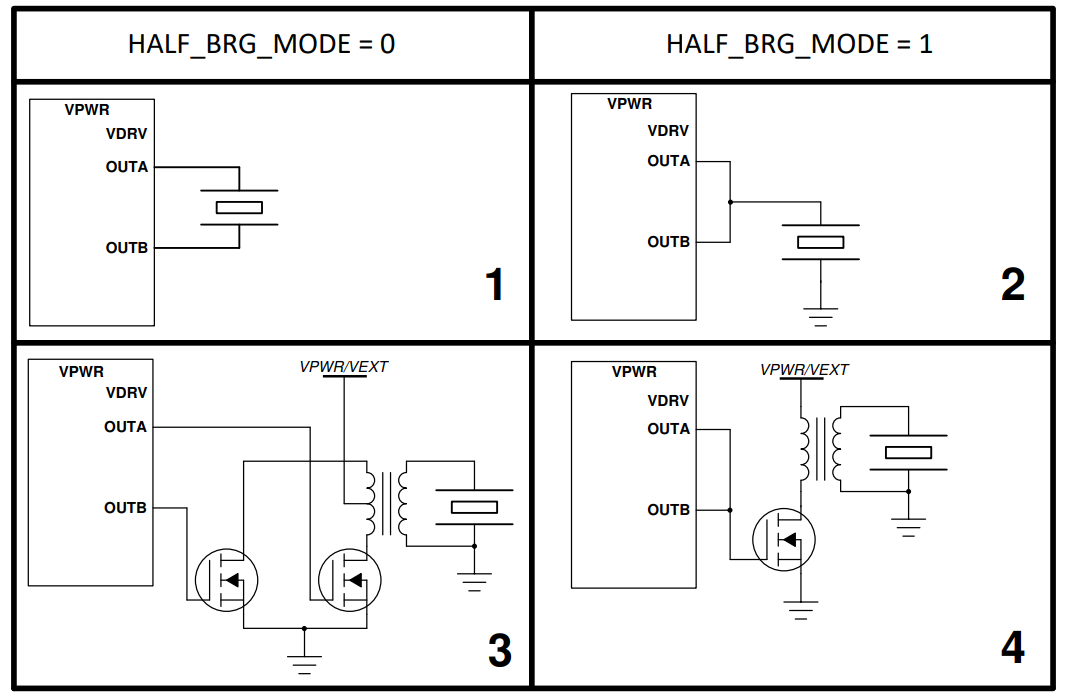
\includegraphics[height=4cm]{figure/TUSS4470 Transducer Drive Options.png}}
    	\hfill
    	\subfloat[实际配置方式]{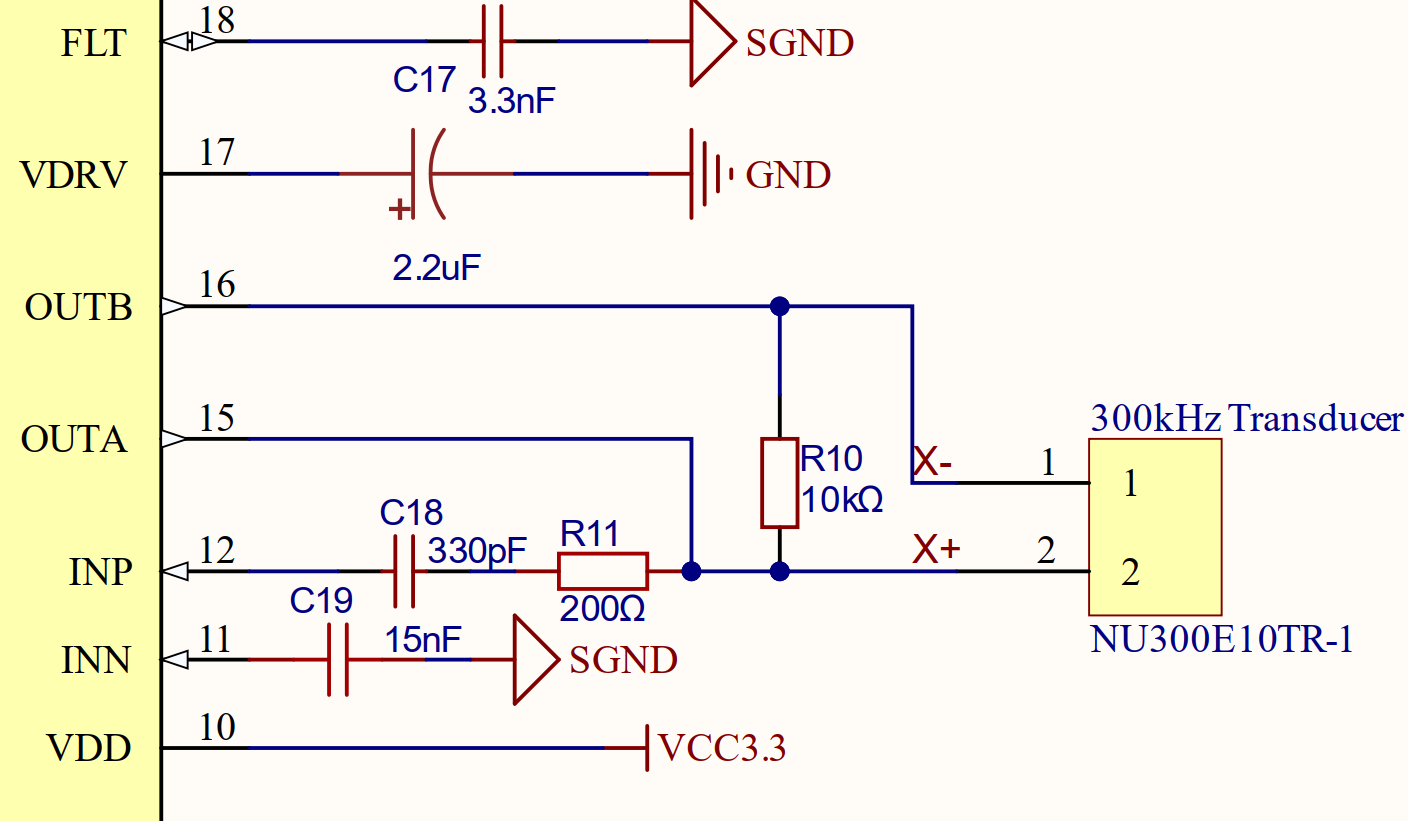
\includegraphics[height=4cm]{figure/OUTA PIN.png}}
    	\hfill
    	\caption{超声换能器驱动电路设计}    %大图名称
    	\label{超声换能器驱动电路设计}    %图片引用标记
    \end{figure}


    \subsubsection{回波检测电路}
    回波检测电路有INP和INN引脚组成,其中INP引脚作为回波检测的正极,INN作为负极连接SGND引脚来进行接地。

    \subsubsection{芯片配置指示电路}
    CPLD芯片通过SPI协议向TUSS4470芯片发送配置数据,并接收其反馈回数据。在芯片返回的数据当中,有一位的状态位用来反映芯片是否准备就绪,当芯片准备就绪后该位置1,可供MCU进行下一步的工作。如图为芯片配置指示电路,当芯片配置就绪后,MCU该引脚拉高,LED灯亮,用来指示芯片的配置状态。
    
    \subsubsection{分离接地电路}
    由于外围电路中包含多种类型的信号,例如VPWR引脚的电源信号,VOUT引脚的模拟信号,VOUT引脚的模拟信号,SCLK等引脚的数字信号。当产生数字信号的引脚产生脉冲时,其变换速度较快,将会在数字地产生较大的噪声;而模拟信号又容易受到外接的干扰,如果将数字信号和模拟信号直接接入同一个大地,将会严重影响模拟信号的准确性,对于超声波传感器而言,是非常致命的。本设计在原理图设计的过程中便解决了不同类型分离接地\upcite{分离接地}的问题,采用的方法是:先将不同类型的信号连接到0$\Omega$电阻,再连接到大地,0$\Omega$电阻相当于很窄的电容通道,能够有效的限制环路电流,使噪声得到抑制。起分离接地作用的电路如\ref{分离接地电路}所示。
     \begin{figure}[ht]
        \centering
        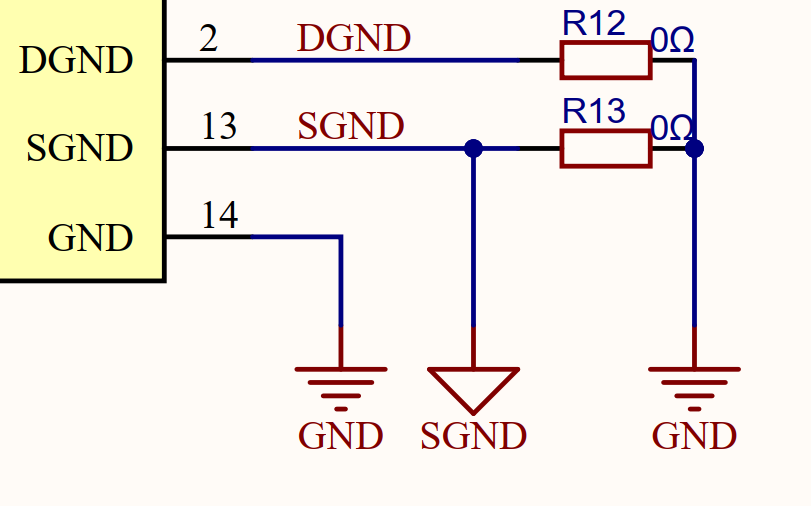
\includegraphics[width=10cm]{figure/seperate ground.png}
        \caption{分离接地电路}
        \label{分离接地电路}
    \end{figure}


    

    
    \subsection{PCB设计}
    由于本设计中涉及到的信号类型较多,包括了数字信号、模拟信号、高频信号、大功率信号,各信号间会存在较大的干扰,因此在布线过程中将各信号分离十分重要,直接关系到传感器的稳定性和精度。如图\ref{传感器PCB设计图}为传感器整体的PCB设计图,本设计采用两层板来完成布线。
      \begin{figure}[ht]
        \centering
        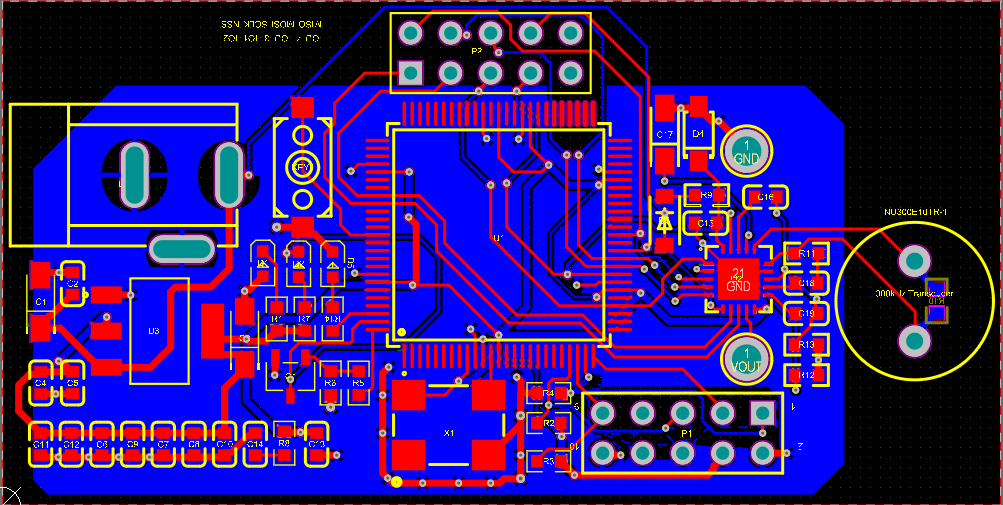
\includegraphics[width=10cm]{figure/overall pcb}
        \caption{传感器PCB设计图}
        \label{传感器PCB设计图}
    \end{figure}
    
    \subsubsection{CPLD芯片部分}
    \noindent
    \textbf{1、线宽}\par
    对于功率较大的部分如电源、超声换能器驱动部分,需要对布线进行加宽处理,避免因发热而影响电路板正常工作,甚至产生损坏。\par
    \noindent
    \textbf{2、时钟}\par
    对于速率较低的时钟,需进行包地处理。包地的作用主要有两点:一是拉开与其他信号的距离,从而减小干扰;二作为自身参考和屏蔽。包地处理还需要在地线上等间距打过孔,如图\ref{时钟包地处理}所示。
     \begin{figure}[ht]
        \centering
        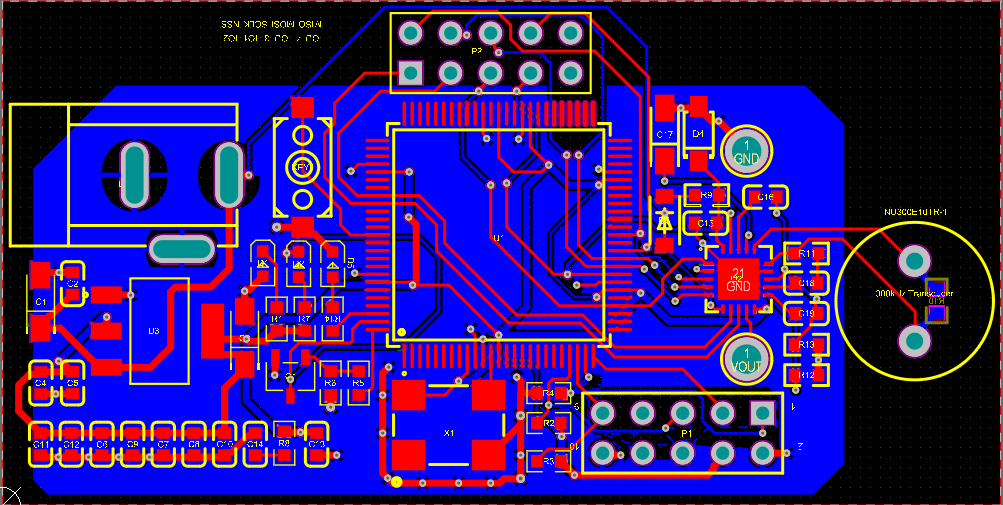
\includegraphics[width=10cm]{figure/overall pcb}
        \caption{时钟包地处理}
        \label{时钟包地处理}
    \end{figure}
    
    
    \subsubsection{TUSS4470驱动芯片部分}
    在TUSS4470驱动芯片的PCB设计过程中,最重要的就是将芯片的电源信号、数字信号以及模拟信号进行分离。参考芯片手册\upcite{TUSS4470芯片手册},在布线时考虑到了如下事项。\par
    \noindent
    \textbf{1、分离接地}\par
    在连接到主地前,数字接地、传感器接地、回波接地都要先通过0$\Omega$电阻或者铜迹线,如图\ref{分离接地电路},本设计在原理图设计时采用了0$\Omega$电阻的方式来实现分离接地,因此在布线时就不需要考虑该问题。
         
     \noindent
    \textbf{2、回波接收引脚}\par
    INN、INP引脚作为回波信号的接收引脚,对噪声干扰十分敏感,所以其布线必须要短且直,并且保证INN引脚的电容尽量靠近芯片引脚,以减少干扰,但考虑到后续需手工焊接,电容与芯片引脚间仍要保持一定的间隙,以减小手工焊接的难度,如图\ref{回波接收引脚}所示。假设不考虑测试成本,采用贴片工艺,电容与芯片引脚间的距离还可再进一步减小,以获得到具有更高稳定性的回波信号。
              \begin{figure}[ht]
        \centering
        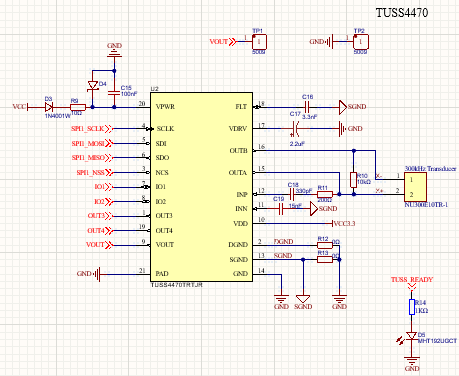
\includegraphics[width=10cm]{figure/TUSS4470 peripheral circuit.png}
        \caption{回波接收引脚}
        \label{回波接收引脚}
    \end{figure}
     \noindent
    \textbf{3、VOUT引脚}\par
    VOUT引脚作为模拟信号输出端,与外界的连线应该尽量短直,避免产生寄生效应\upcite{寄生效应},以及外部噪声干扰引起的噪声耦合\upcite{噪声耦合}。\par
     \noindent
    \textbf{4、超声换能器驱动}\par
    芯片与OUTA、OUTB引脚间的布线应尽可能短且直,以保证发出脉冲信号的质量,从而提高传感器的精度。考虑到两个引脚输出的是大功率、高频率的模拟信号,连接到两引脚的线宽应不能太小。\par
    \noindent
     \textbf{5、VPWR引脚}\par
        根据芯片手册推荐,VPWR的解调电容应尽可能靠近引脚。\par
     \noindent
    \textbf{6、信号分离}\par
     数字信号引脚如TXD、RXD、 SCLK、 NCS、 
IO1、 IO2、 OUT3、OUT4应远离模拟信号引脚,避免信号间的干扰。\par
\subsection{本章小结}
至此已介绍完成传感器硬件部分的设计过程及说明,下一章将详细讲解传感器的程序设计部分。

      
    
    
    